
\chapter{Introduction}

This document gently introduces to the preparation of standalone Web Services and cognate clients with the Advance Resource Connector (ARC).
The reader is guided through a series of practically oriented examples.
Each is accompanied by explanations of the main concepts of the software architecture.
No particular skills are required to follow the presented steps.
It is however beneficial to have some basic comprehension of the programming language C++, the file format XML and any regular UNIX shell.
To start, the user shall have an installation of ARC-1, as it is performed with current RPM or .deb packages\footnote{see http://wiki.nordugrid.org for explicit instructions for setup}.


The ARC server provides access to services.
These are executed on the same machine that the server is installed on.
Some services, like the a-rex service, will delegate computational efforts to other machines
via additional software like a local queueing system.
But the a-rex service itself does not migrate away to other machines - at least this
has not been implemented yet.
Services may comprise computational tasks (e.g., some secret and strongly
patented algorithm), allow arbitrary computations (like ARC's a-rex or
Amazon's clouds) or provide access to other resources like a particular
database or to arbitrary disk space (like ARC's hopi or bartender).


The users of computational services are software tools, too.
They are referred to as clients.
It is those clients that perform the interactions with a human user.
However, when a service requests a performance of another service at the same or another server, then this first service is in the role of a client, too.


Servers provide access to a single service or a set of services. For ARC, there is one service, named Hosting Environment Demon (HED), more special than other services: HED organises the assignment of other services on the same server to the network. But this does not break the concept, it is only a commodity. If services are not busy reacting to a client's request, then they are waiting. The task of servers can be subdivided into:
\begin{itemize}
 \item Wait for client request
 \item Receive the request
 \item Perform the desired service
 \item Create a response for the client
 \item Send response to the client
 \item Wait for next client request
\end{itemize}
While the server waits passively for a request, the client acts actively:
\begin{itemize}
 \item Create a request
 \item Transmit the request to the server which provides the desired service.
 \item Wait for the reply
 \item Receive the response from the server.
 \end{itemize}
\forcelinebreak

In general, the implementation of a client is easier than the implementation of the server. 
ARC is designed as a middleware which encapsulates typical challenges of server-client infrastructures (security, exception handling, extensibility) and abstracts from the underlying computer architecture (heterogeneity of computers, computer location, protocols).
The core of ARC is the prior mentioned HED (Hosting Environment Daemon).
To the administrator HED is mostly visible as the single binary that is started and configured by a file that describes services that shall be prepared by HED. 
Conceptionally, the HED determines how services shall be organised both as a principle, and for any given ARC-run server.
HED determines the very explicit presence or absence of a service at a particular address. Its many configurable layers are described later in this tutorial. 
%
At the time of writing, the endpoint of the HED will be a SOAP based  Web Service.
SOAP is a long established XML-based standard for Web Service communication.
ARC abstracts from this format, but nevertheless it is useful to be aware of
the underlying message transport mechanism.

%which implicate several advantages.
%The XML file format is not restricted to a certain set of tags but can be expanded in such a way as to fit almost any kind of service. It is not a proprietary format and as a result many libraries in almost any language are capable in creating that kind of format.Likewise, XML is also suitable for the usage between heterogeneous platforms.However, while the client can be implemented very straight, the service has to fit a certain layout.In the present guide four kinds of webservices will be introduced: a simple time service, an echo service, a secure echo service and a service with a persistence state .\\


 


\section{Hosting Environment Daemon}

The HED which was already mentioned in the section above is an essential part of the ARC middleware. 
Its task is to provide the hosting of various services at the application level and is based on the idea modularity. % allows its dynamic extension.
The HED consists of components called Message Chain Components (MCC), Plexer, Services, and several modules, which shall aid the programmer to simplify the development of the Web Services: Config, Loader, Logging, XMLNode et cetera.
The MCCs are ordered within a layered structure. 
Each MCC provides a certain functionality such as communication between two applications (MCC TCP), secure data transfer (MCC TLS) or client-server architecture (MCC HTTP).
Figure~\ref{fig:HED_internal} illustrates a typical setup of a server-sided HED.

\begin{figure}[htb]
	\centering
	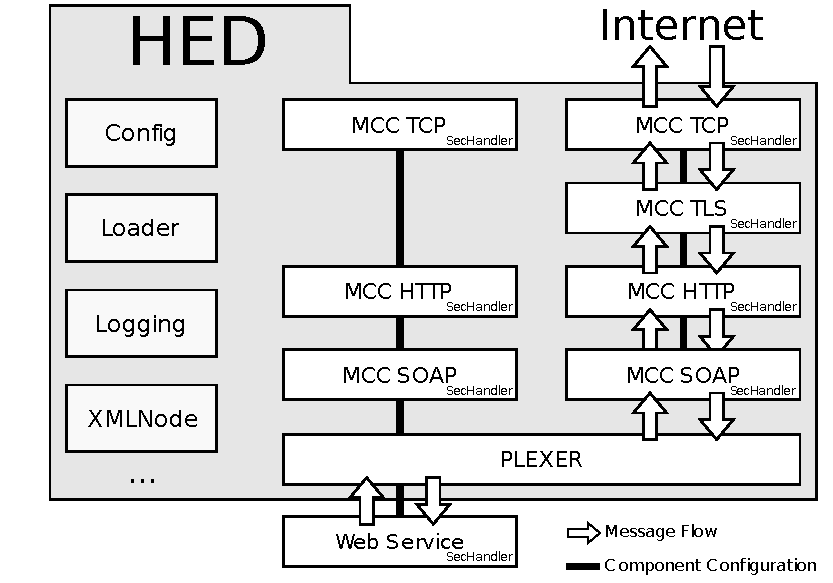
\includegraphics[width=14cm]{tex_introduction/HED2.pdf}
	\mycaption{Example of a HED structure providing a Web Service}{The HED consists of several layers which are connected with each other. The arrow indicate the message flow of the used configuration. The MCCs and Services may hold a SecHandler in order to give additional security. Additional modules (on the left) are used within the HED. \task{Why is the Web Service in all images outside of the HED?}}
\label{fig:HED_internal}
\end{figure}

As to be seen, the MCCs are connected which each other and passing incoming and outgoing message to the upper or the respective lower layer. In case of outgoing messages a MCC is wrapping the data of the upper layer as a payload into their own protocol (while incomming message will be unwrapped).
The lowest layer has to be a transport protocol like TCP which enables the transmission between two applications.
Technically there even lower layers required needed for the communication but they are already realised within the operating system and the  network card.
TCP is well suited for the application because it provides a reliable and ordered delivery of a byte stream.
Above the TCP layer is the Hypertext Transfer Protocol (HTTP). 
In case a security layer is desired (i.e. for authentication), the TLS (Transport Layer Security formerly known as SSL, Secure Sockets Layer) has to be inserted between the TCP and HTTP layers.
The HTTP provides the client-server architecture. It is stateless but offers several extensions for requests, header information and status codes. Furthermore HTTP enables the usage of Uniform Resource Locators (URL) which is used by ARC to multiplex between different services. The multiplexing layer can also be defined within the HED and is called Plexer.
Depending on the path of the URL the Plexer passes messages to a defined SOAP service which again passes the message to the Web Service~\cite{QIANG_2005}.\\
% QUESTION: Why is the plexer always illustrated  being above the SOAP MCC. There's no config file example like that in the tree.
%In my understanding (because plexer is not my initial idea), plexer (as a sort of hub) can be put at both after http or soap. If you put after soap,then you are doing switching for different web services. While I put it after http, because somehow, I need to switch the message after http-processing, in more detail, one branch for soap and then web service/s, one branch for a non-soap service/server (the SP Service is not a service based on SOAP, actually it is based on http, so it is kind of web application).


The structure of the HED can be configured freely by modifying the server configuration file.
A first impression how the HED can be configured shall be given in the following example which corresponds to the HED shown in Figure~\ref{fig:HED_internal}.
It uses the ARC echo service that is shipped for testing purposes with the ARC source code.



\subsection{The ARC echo service}


The first example shall give a basic understanding in how to configure the HED for setting up a novel service.
The task will be to setup the regular ARC Echo Web Service.
On the command line, all that needs to be done is to invoking the \textit{arched} daemon with a fitting server configuration file.
Such a fitting server configuration file is shown in Listing~\ref{lst:arched_arcecho_xml}.
It is written in XML. Its structure is based on the XSD schema listed in~\ref{sec:impXSD} in Listing~\ref{lst:mcc.xsd}.\\ 

\lstsetARCHEDXML
\lstinputlisting
	[label=lst:arched_arcecho_xml,float=htb,
	caption={[HED configuration file.]
	\textbf{HED configuration file.}}]
{../src/services/arched_arcecho.xml}
The first line of the XML file contains the XML declaration.
Several attributes can be defined here but at least the XML version should be specified.
The configuration as a whole is encapsulated by the element \textit{ArcConfig}. It also performs the setting of namespace abbreviations, which are expected to be mostly invariant across all server installations.% ABBREVIATIONS?? - MG
The \textit{Server} element, to be found at line~\ref{lst_code:arched_arcecho_Server}, provides basic settings for the daemon such as location of the Pid-file or the Log-file.
The \textit{ModuleManager} holds the path to the plugin libraries.
Several paths may be defined here.
Due to the fact that the first library fitting to the plugin name is loaded, the order is relevant.
The path should be at least assigned to the ARC installation directory.
Otherwise, the standard set of MCC modules might not be found.
The next set of elements are holding the name of the plugins to be loaded (line~\ref{lst_code:arched_arcecho_Plugins}).
The names have to correspond to the name of the dynamic libraries within the path defined in the \textit{ModuleManager}.
Finally, the chain is declared within the element \textit{Chain} which creates the layered structure.
It is composed of the elements \textit{Component}, \textit{Plexer} and \textit{Service}.
Every element inside has at least a \textit{name} attribute.
Regarding the components and the services a plugin (*.so file found in the paths previously specified) has to be loaded which provides the implementation of its functionality. The further configuration depends on the individual functionality.\\
%
% within the chain ... 3 types of elements
%
%Its needed to distinguish between the plugins and the components.
%The plugins refer to shared libraries that can be integrated as modules with the HED to extend its functionality.
%The Components refer to the implementation of Web Services within any of those libraries.
%
%
A \textit{Chain} will determine the path that an event takes to be noticed.
The first component of the chain is the \textit{tcp.service}.
As to be seen, the port 60000 is assigned to the server to listen to.
The port can be an arbitrary number.
However, the number 60000 is commonly used for a HED providing the A-REX Web Service (the one organising the computation on a site) and the number 50000 is found commonly used for a HED running Web Services for storage.
This way, one can organise a single server to offer multiple HED instances.
The stream which is received by this component is passed to the component defined by the \textit{next} attribute.
In the present case, it will be passed to the component with the \textit{id} attribute named \textit{http}.
In this way, the message is be passed to higher layers until it reaches the \textit{Plexer}.
Depending on the path of the URL which was demanded by the HTTP, the Plexer multiplexes the request to the right Web Service\task{, the right function to execute according to the component IDs and plugin names. -- ??MG}
The plexer will thus allow to have multiple Web Service listen to the same port.
The path, declared within the \textit{next} attribute, corresponds to a regular expression and leads to the service with the id named \textit{echo}. 
Hence, the service will now be reachable under URL \textit{http://localhost:60000/echo}.
It will finally process the message and create a new message which will be returned all the way back to the TCP component.
The Echo Web Service itself is provided by the ARC package.
Additional invariant parameters are passed by the elements \textit{prefix} and \textit{suffix}.
They set the characters which will enclose the echoed string.
\task{The images of the HED structure always are ordered like: TCP - TLS - HTTP - PLEXER - SOAP - Web Service   but the source code examples are: TCP - TLS - HTTP - SOAP - PLEXER - Web Service}

To create the daemon corresponding to the defined server configuration file, ARC provides the program called \textit{arched}.
The manner of invokation is to been seen in Listing~\ref{lst:arcecho_arched_invokation}.
\lstsetKSH
\begin{lstlisting}[
label=lst:arcecho_arched_invokation,float=htb,
caption={[Invokation of the arched daemon in order to start the ARC Echo Web Service.]
         \textbf{Invokation of the Arched Daemon.\textcolor{white}{hmf}}}]

$ arched -c arcecho_no_ssl.xml && echo Daemon started || echo Daemon start failed
 Daemon started
$
\end{lstlisting}

% $ rm -f /var/log/arched.log
% $ tail -n100 -f /var/log/arched.log
%...
%$ killall arched
%
%
The name of the program is followed by the parameter \textit{-c}.
The string following that argument contains the full path of configuration file.
Once the server is running, the client can be used as described in Listing~\ref{lst:arcecho_client_invokation}.
\lstsetKSH
\begin{lstlisting}[
label=lst:arcecho_client_invokation,float=htb,
caption={[Usage of the ARC Echo client.]
         \textbf{Usage of the Arc echo client.\textcolor{white}{hmf}}}]
$ arcecho http://localhost:60000/Echo text
[ text ]
\end{lstlisting}

In this example, the server and the client are running on the same computer such that the hostname \textit{localhost} can be utilized. 
For debugging it is advisable to check the logfile which was assigned inside the server configuration file.
It is commonly found at /var/log/arched.log

The following chapters explain how to develop custom Web Services.
The first one will be the simple Time Web Service.












